\appendix

\section{Difference-in-Difference Question Count Results}\label{app:did}

\begin{figure}[htpb!]
    \centering
    \includesvg[width=1\textwidth]{imgs/pre-post_correlation_matrices.svg}
    \caption{Correlation Matrices Before and After ChatGPT Release}
    \label{fig:app-correlation_matrix}
    % Figure 3 reference
\end{figure}


\begin{figure}[htpb!]
    \centering
    \begin{subfigure}[b]{0.475\textwidth}
        \centering
        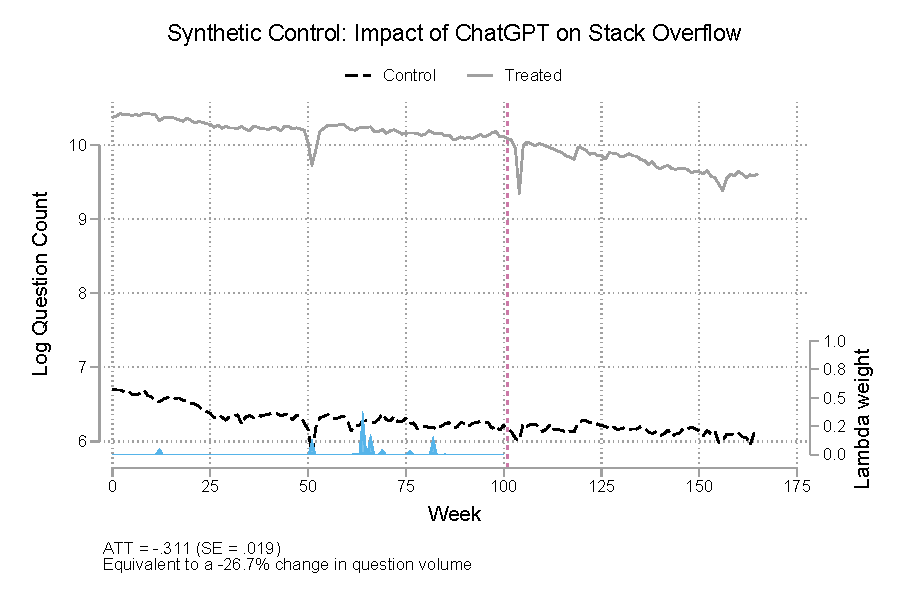
\includegraphics[width=1\textwidth]{imgs/stata/sdid_all_trends101.pdf}
        \caption{Impact on All Stack Overflow Questions}
        \label{fig:app-sdid_all}
    \end{subfigure}
    \hfill
    \begin{subfigure}[b]{0.475\textwidth}
        \centering
        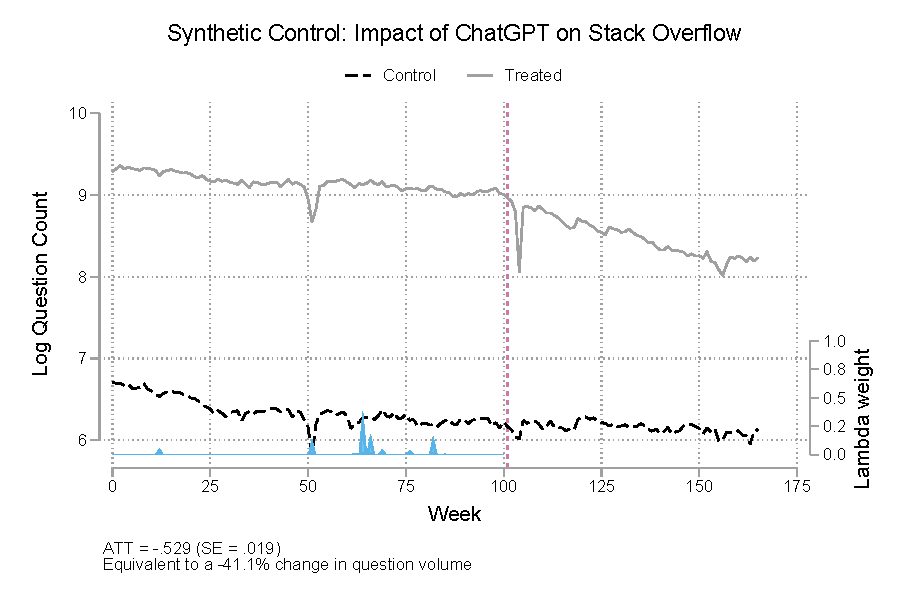
\includegraphics[width=1\textwidth]{imgs/stata/sdid_script_trends101.pdf}
        \caption{Impact on Scripting Language Questions}
        \label{fig:app-sdid_script}
    \end{subfigure}
    \caption{Synthetic difference-in-difference plots}
    \label{fig:app-DiD}
\end{figure}

\begin{table}[htpb!]
    \centering
    \caption{Synthetic DiD Estimates of ChatGPT's Impact on Stack Overflow Question Volume}
    \label{tab:app-sdid_results}
    \begin{tabular}{lcccc}
        \toprule
            & \multicolumn{2}{c}{All Questions} & \multicolumn{2}{c}{Scripting Languages} \\
            \cmidrule(lr){2-3} \cmidrule(lr){4-5}
            & (1) & (2) & (3) & (4) \\
        \midrule
            Treatment Effect & $-0.311^{***}$ & $-0.308^{***}$ & $-0.502^{***}$ & $-0.497^{***}$ \\
            & $(0.019)$ & $(0.000)$ & $(0.042)$ & $(0.039)$ \\
        \midrule
            Month covariates & No & Yes & No & Yes \\
            Percent Change & $-26.7\%$ & $-26.5\%$ & $-39.5\%$ & $-39.2\%$ \\
        \midrule
            Observations & 830 & 830 & 1,328 & 1,328 \\
            Number of groups & 5 & 5 & 8 & 8 \\
            Pre-treatment periods & 101 & 101 & 101 & 101 \\
            Post-treatment periods & 65 & 65 & 65 & 65 \\
        \bottomrule
            \multicolumn{5}{p{0.95\linewidth}}{\footnotesize \textit{Notes:} Standard errors in parentheses based on placebo/bootstrap replications (100 repetitions). $^{***}p<0.001$. The dependent variable is log question count. All models include time and group fixed effects. Treatment is defined as the period after ChatGPT's release (November 30, 2022).} \\
    \end{tabular}
\end{table}

\begin{figure}[H]
    \centering
    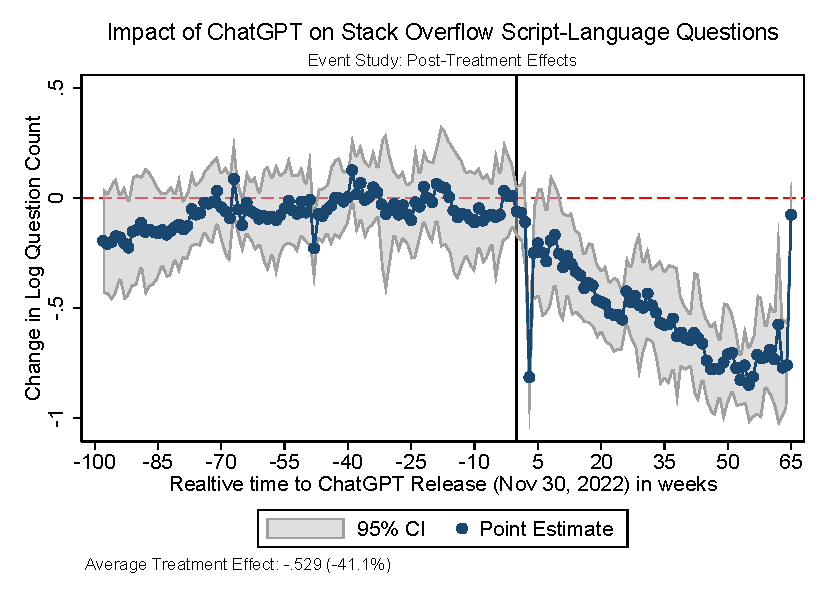
\includegraphics[width=0.9\textwidth]{imgs/stata/event_study_scripting_languages.pdf}
    \caption{Event Study Analysis for Scripting Language Questions}
    \label{fig:app-event_study}
\end{figure}

\section{Processing Pipeline}\label{app:procpipe}

\begin{figure}[htpb!]
    \centering
    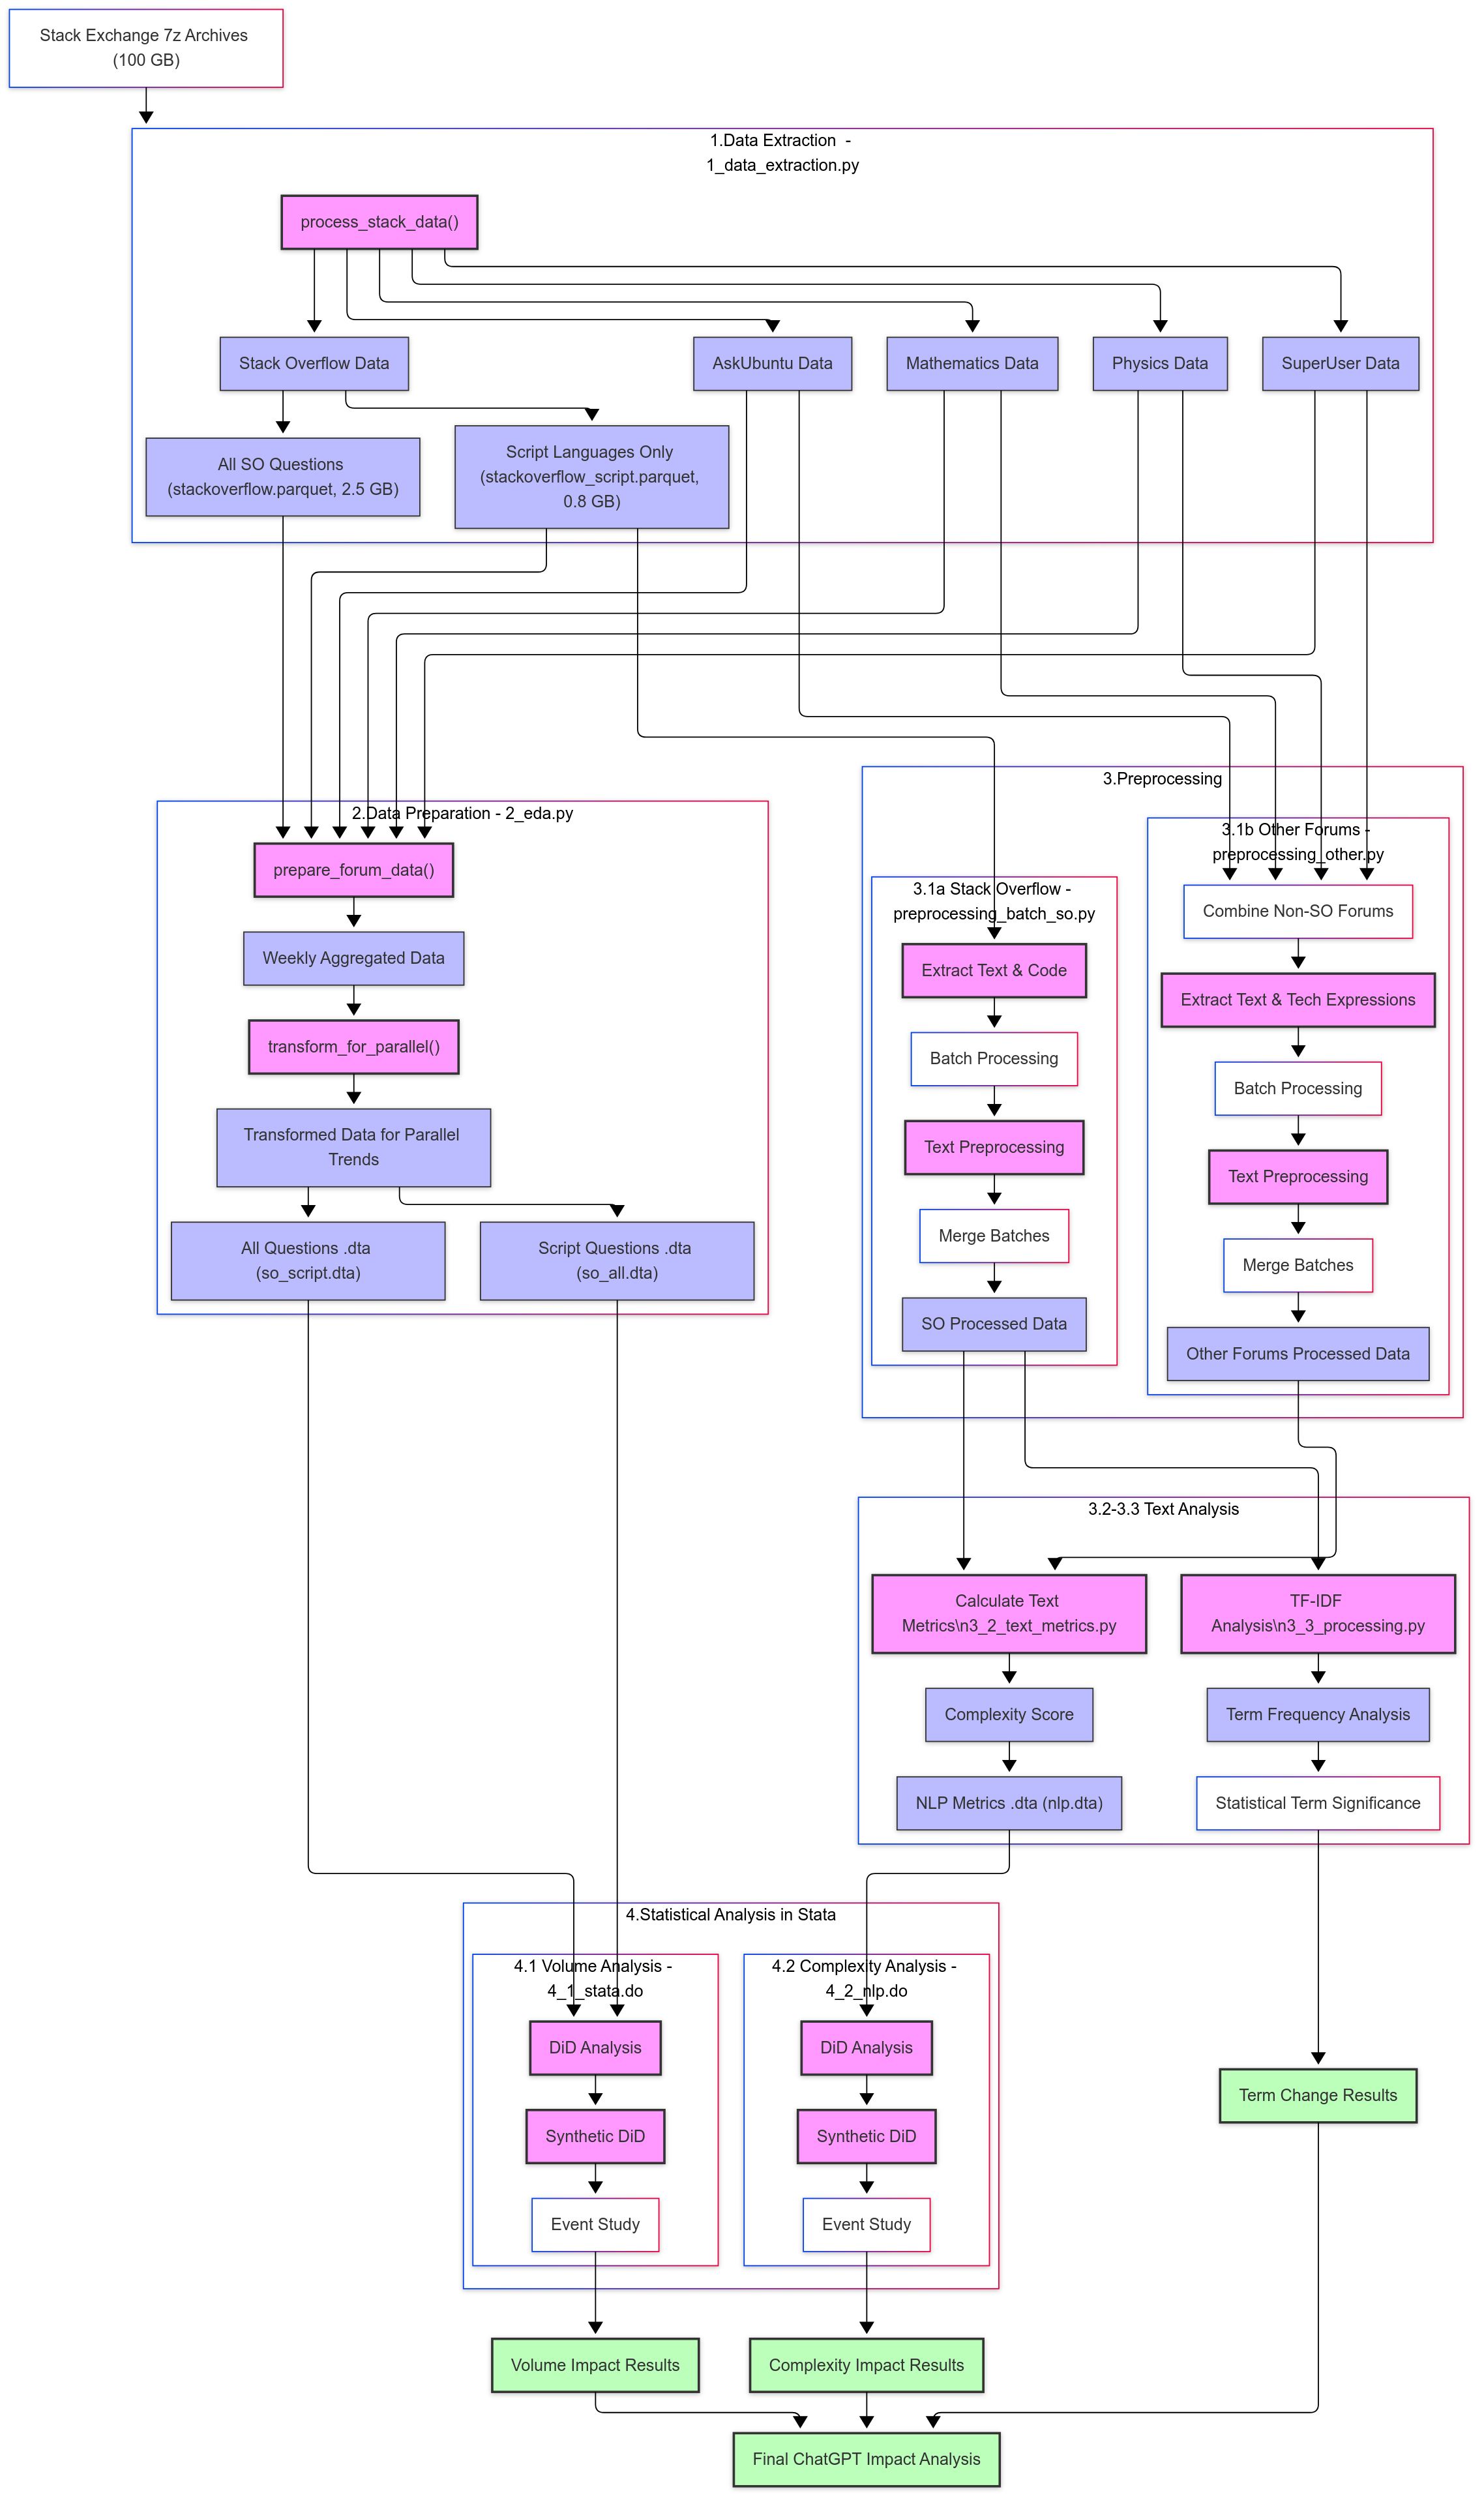
\includegraphics[width=1\linewidth]{imgs/process_flow.png}
    \caption{Sketched process and file flow}
    \label{fig:app-process_flow}
\end{figure}


\section{Difference-in-Difference Complexity Score Results}\label{app:did}